
\section{Initialisation du programme}
\label{scenarii:init}
    
Lors de l'initialisation du programme, trois cas de figure peuvent être
rencontrés : 

\begin{itemize}
\item L'initialisation se passe correctement et le programme est prêt à être
utilisé.
\item Une erreur est introduide à cause d'un échec de connexion à la base de
données.
\item Une erreur est introduite à cause d'un échec de connexion au module de
sortie.
\end{itemize}

\subsection{Initialisation réussie}
\label{scenarii:init:reussie}

Lors du démarrage du programme, l'interface utilisateur va demander au 
module de génération de playlists de vérifier la présence d'une base de 
données accessible. La rêquete est alors transmise du générateur au module 
de données qui va effectuer une connexion avec la base de données.
        
Une fois cette connexion correctement effectuée, le module de données va 
faire remonter l'information au générateur qui va, à son tour, la 
transmettre à l'interface utilisateur.

Ensuite, l'interface utilisateur s'assure qu'il y ait au moins un module de 
sortie fonctionnel en récuperant une liste des différentes sorties possibles.

Enfin, l'interface utilisateur s'adapte pour correspondre aux services de 
sortie disponibles.
        
\begin{figure}[H]
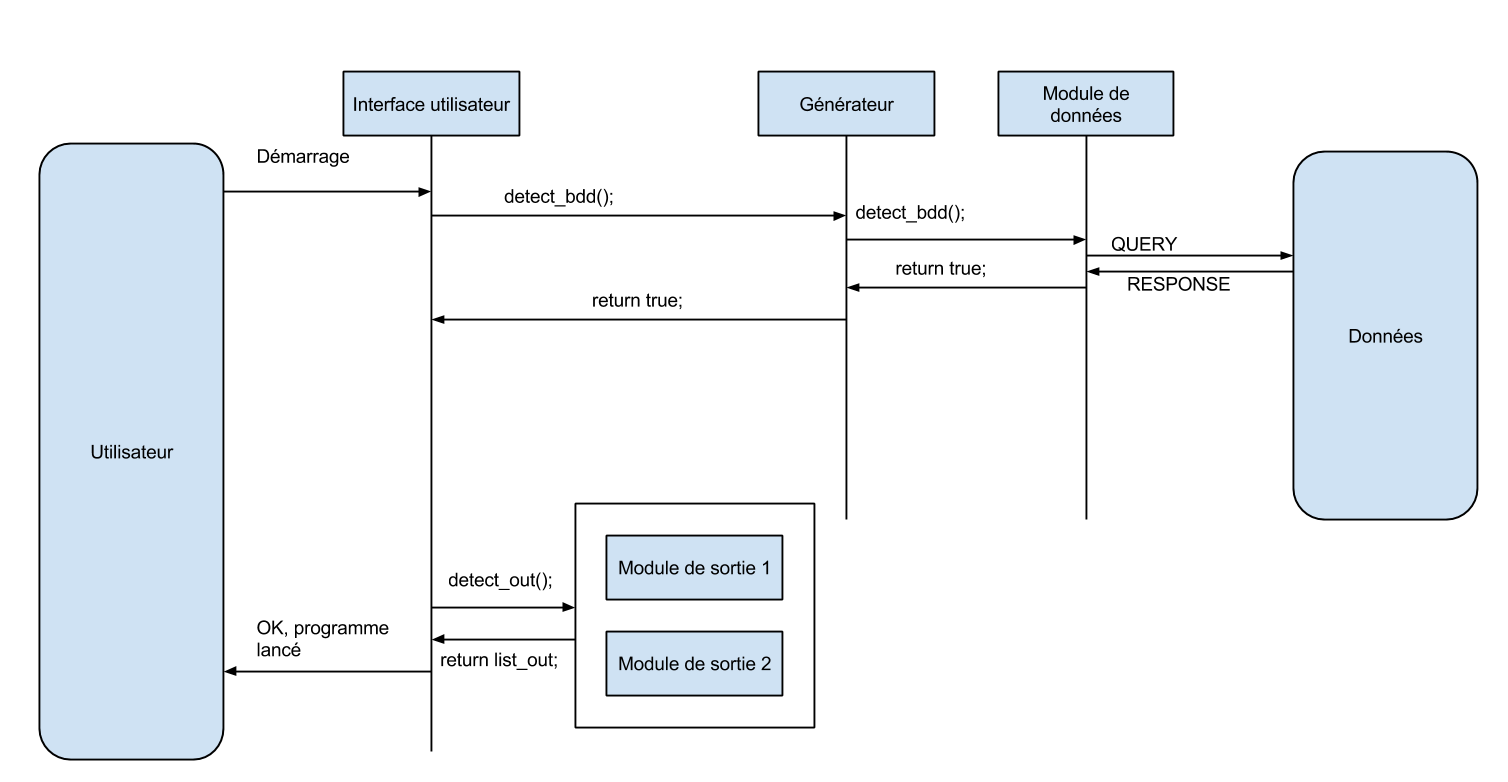
\includegraphics[width=\textwidth]{data/scenarii/demarrage_fonctionnel.png}
\caption{Initialisation réussie, le programme est lancé.}          
\end{figure}
        
\subsection{Absence de base de données}
\label{scenarii:init:nobdd}
        
Lorsque le module de données tente de se connecter à la base de données, il 
se peut que la connexion échoue pour diverses raisons. Dans ce cas, le 
module de données renvoie au générateur un message d'erreur qu'il transmet à
 l'IHM, afin de l'afficher pour avertir l'utilisateur de cette erreur. Puis 
 le programme s'arrête.
        
\begin{figure}[H]
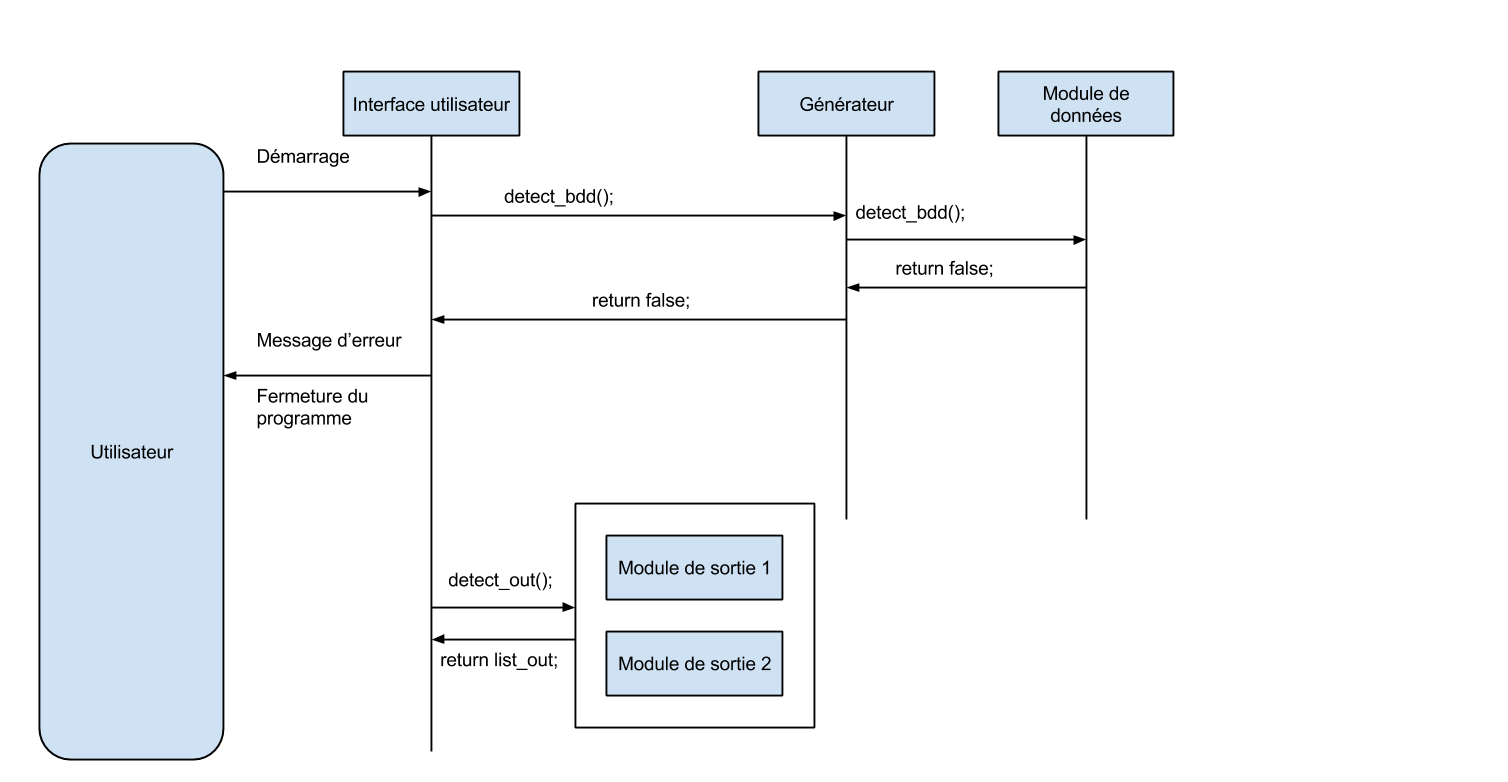
\includegraphics[width=\textwidth]{data/scenarii/demarrage_absence_bdd.png}
\caption{Absence de base de données lors de l'initialisation}
\end{figure}
        
\subsection{Absence de module de sortie}
\label{scenarii:init:noout}

Dans le cas où l'interface utilisateur effectue correctement une connexion à 
la base de données, mais n'arrive pas à établir une liste des sorties 
disponibles (à cause d'une absence du module de sortie ou d'aucune sortie 
disponible), elle doit afficher un message d'erreur à l'attention de 
l'utisilateur, et entraîner l'arrêt du programme.
        
\begin{figure}[H]
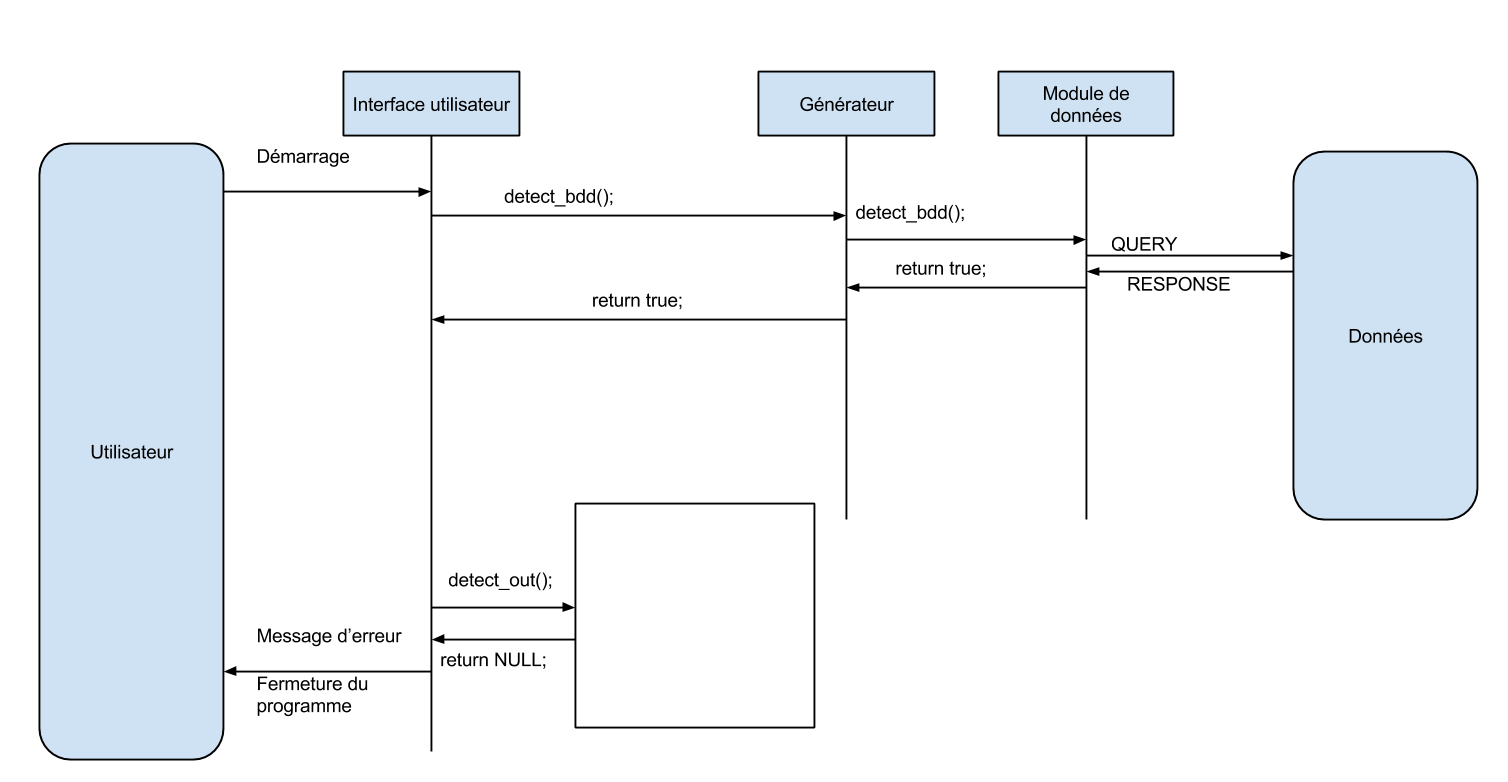
\includegraphics[width=\textwidth]{data/scenarii/demarrage_absence_sortie.png}
\caption{Absence de sorties disponibles lors de l'initialisation}
\end{figure}
 
\section{Génération}
\label{scenarii:gen}

\subsection{Génération fonctionnelle et satisfaisante}
\label{scenarii:gen:satis}

\begin{enumerate}
\item L'utilisateur décide de lancer la génération d'une playlist.
\item Le module d'interface utilisateur appelle le module de génération et 
lui transmet les paramètres entrés par l'utilisateur.
\item Le module de génération appelle le module de données et lui transmet 
une requête de morceaux satisfaisant les paramètres choisis par l'utilisateur.
\item Le module de données lance les requêtes SQL sur la base de données et
récupère les informations renvoyées.
\item Ces informations sont rendues au module de génération puis sont 
utilsées pour créer une liste de morceaux.
\item Le module de génération calcule la bonne similarité de la playlist.
\item Le module de génération renvoie la playlist ainsi crée à l'interface 
utilisateur qui la passe au module de sortie demandé.
\item Ce module génére la sortie et la rend directement à l'utilisateur en 
passant par l'interface.
\end{enumerate}

\begin{figure}[H]
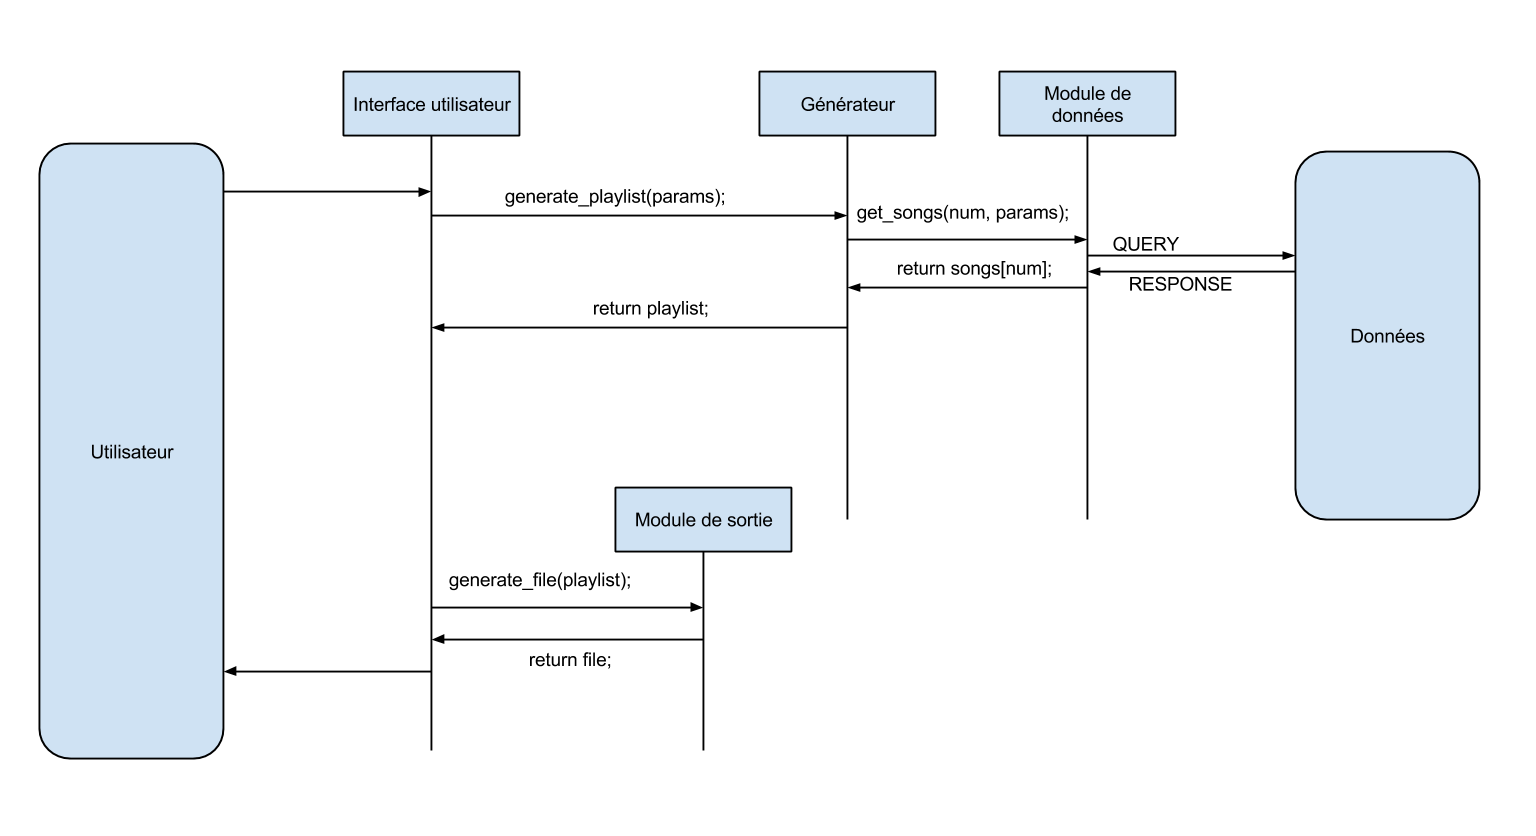
\includegraphics[width=\textwidth]{data/scenarii/generation_fonctionnel.png}
\caption{Génération de playlist réussie}
\end{figure}

\subsection{Génération non satisfaisante}
\label{scenarii:gen:nosatis}

\begin{enumerate}
\item L'utilisateur décide de lancer la génération d'une playlist.
\item Le module d'interface utilisateur appelle le module de génération et 
lui transmet les paramètres entrés par l'utilisateur.
\item Le module de génération appelle le module de données et lui transmet 
une requête de morceaux satisfaisant les paramètres choisis par l'utilisateur.
\item Le module de données lance les requêtes SQL sur la base de données et
récupère les informations renvoyées.
\item Ces informations sont rendues au module de génération puis sont 
utilsées pour créer une liste de morceaux.
\item Le module de génération calcule la bonne similarité de la playlist, 
mais celle ci ne répond pas aux attentes.
\item Le module de génération renvoie la playlist à l'IHM qui demande à 
l'utilisateur s'il veut affiner la recherche ou non.
\item Si oui, on lance une nouvelle génération en gardant la liste générée 
au passage précédent (On répète les étapes 3, 4, 5 et 6). Si non, on passe 
directement à l'étape suivante.
\item Le module de génération renvoie la playlist ainsi crée à l'interface 
utilisateur qui la passe au module de sortie demandé.
\item Ce module génére la sortie et la rend directement à l'utilisateur en 
passant par l'interface.
\end{enumerate}

\begin{figure}[H]
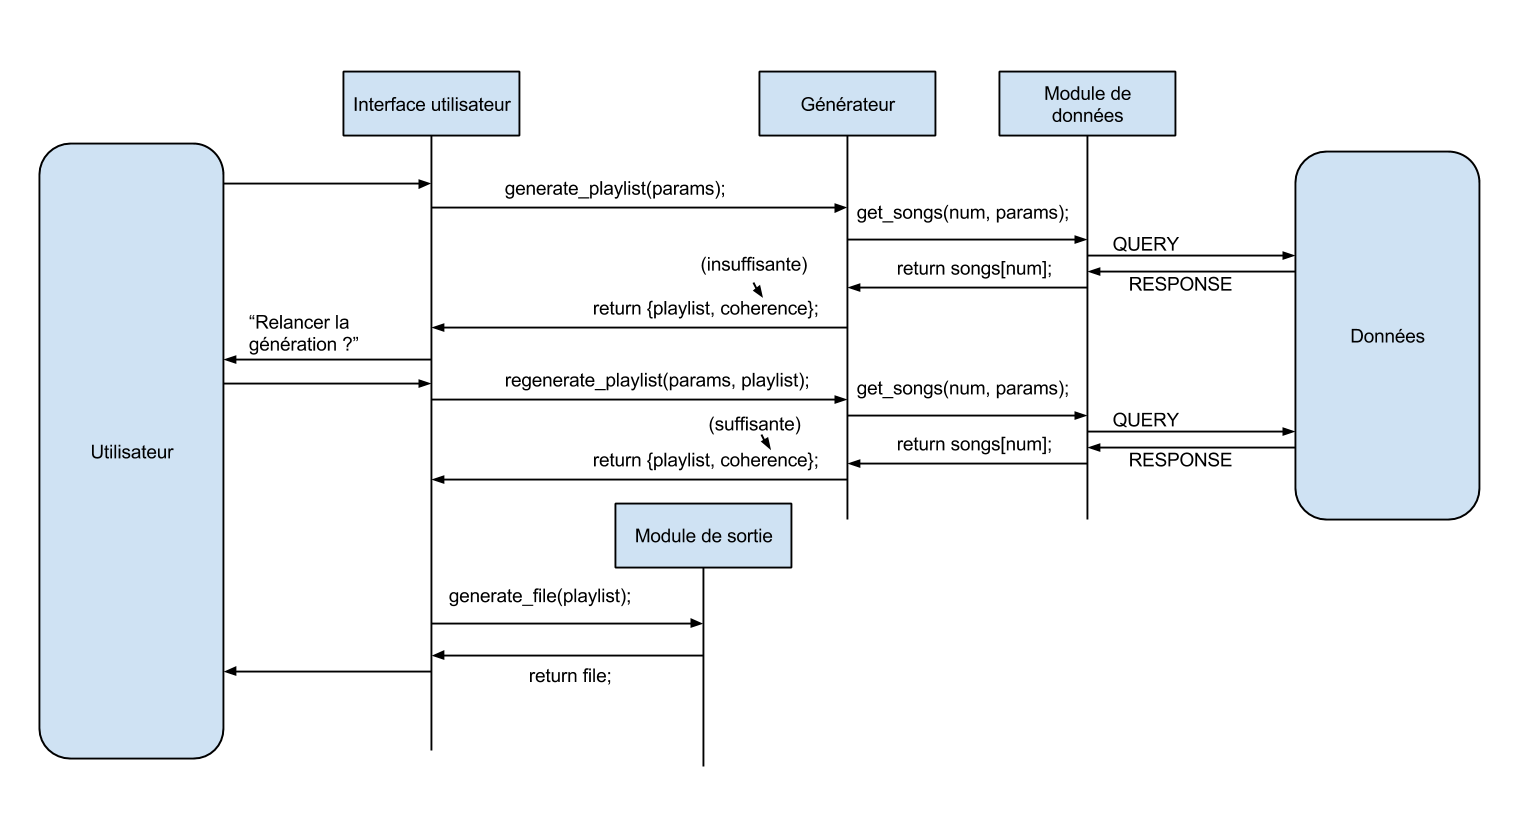
\includegraphics[width=\textwidth]{data/scenarii/generation_decevante.png}
\caption{Génération de playlist non staisfaisante, l'utilisateur relance la génération}
\end{figure}
 

\subsection{Génération incomplète}
\label{scenarii:gen:incomp}

\begin{enumerate}
\item L'utilisateur décide de lancer la génération d'une playlist.
\item Le module d'interface utilisateur appelle le module de génération et 
lui transmet les paramètres entrés par l'utilisateur.
\item Le module de génération appelle le module de données et lui transmet 
une requête de morceaux satisfaisant les paramètres choisis par l'utilisateur.
\item Le module de données lance les requêtes SQL à la base de données et
récupère les informations, mais il n'y a pas assez de morceaux correspondant 
aux critères demandés par l'utilisateur.
\item Ces informations sont rendues au module de génération puis sont 
utilsées pour créer une liste de morceaux.
\item Le module de génération calcule la bonne similarité de la playlist.
\item Le module de génération renvoie la playlist ainsi crée à l'interface 
utilisateur.
\item L'IHM avertit l'utilisateur que la playlist est incomplète avant de 
passer la playlist au module de sortie demandé.
\item Ce module génére la sortie et la rend directement à l'utilisateur en 
passant par l'interface.
\end{enumerate}

\begin{figure}[H]
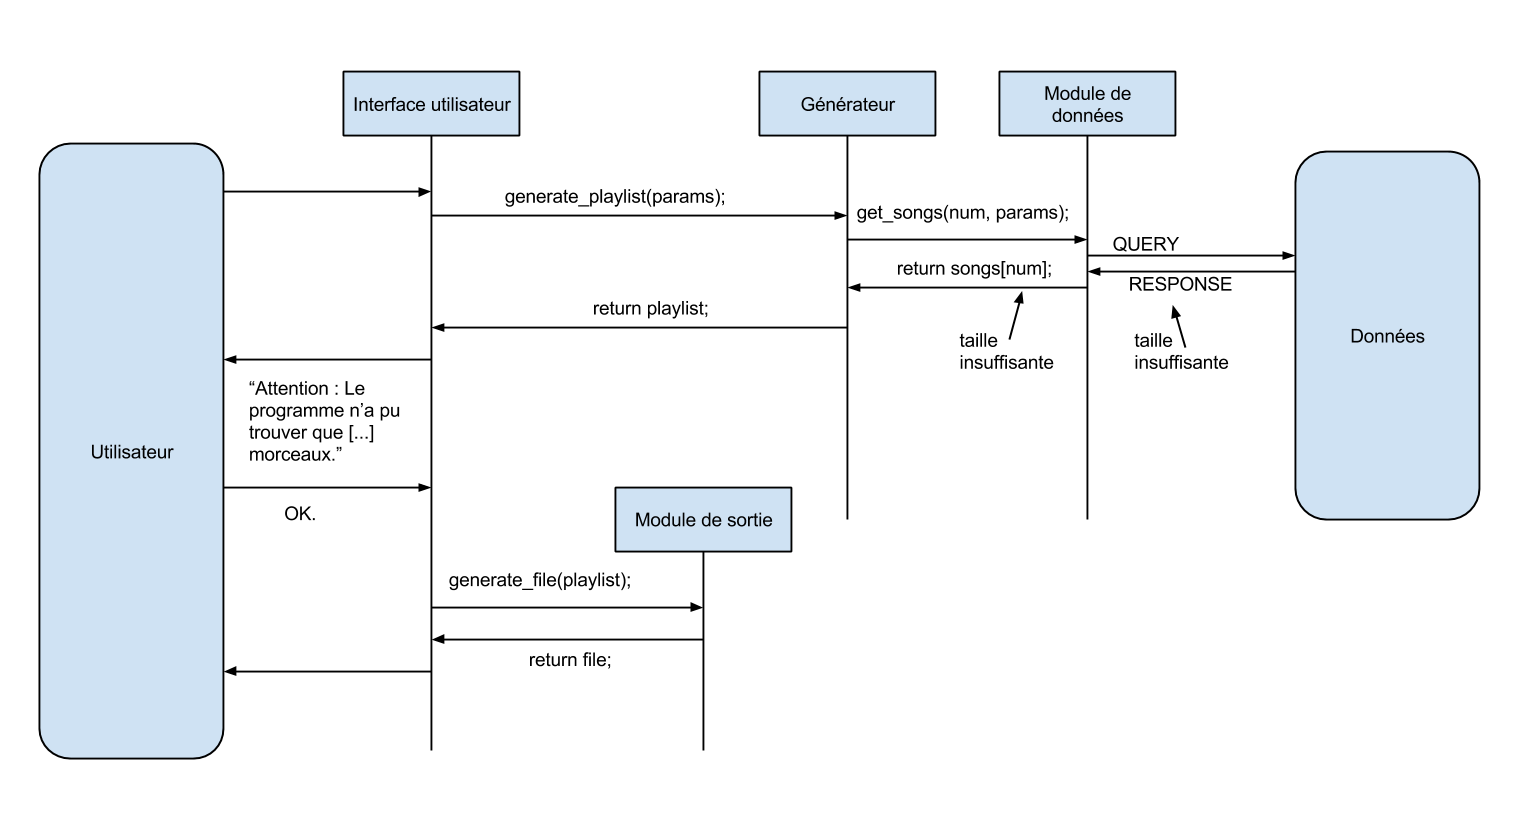
\includegraphics[width=\textwidth]{data/scenarii/generation_incomplete.png}
\caption{Génération terminée mais incomplète, on avertit l'utilisateur}
\end{figure}
 

\subsection{Absence de données répondant aux paramètres}
\label{scenarii:gen:nodata}

\begin{enumerate}
\item L'utilisateur décide de lancer la génération d'une playlist.
\item Le module d'interface utilisateur appelle le module de génération et 
lui transmet les paramètres entrés par l'utilisateur.
\item Le module de génération appelle le module de données et lui transmet 
une requête de morceaux satisfaisant les paramètres choisis par l'utilisateur.
\item Le module de données lance les requêtes SQL à la base de données mais 
ne récupère pas d'informations : il n'y a pas de morceaux correspondants aux 
critères demandés par l'utilisateur.
\item Le module de génération renvoie une liste vide à l'interface 
utilisateur.
\item L'IHM avertit l'utilisateur que la requête ne renvoie aucune 
information et qu'aucune playlist ne peut être générée.
\end{enumerate}

\begin{figure}[H]
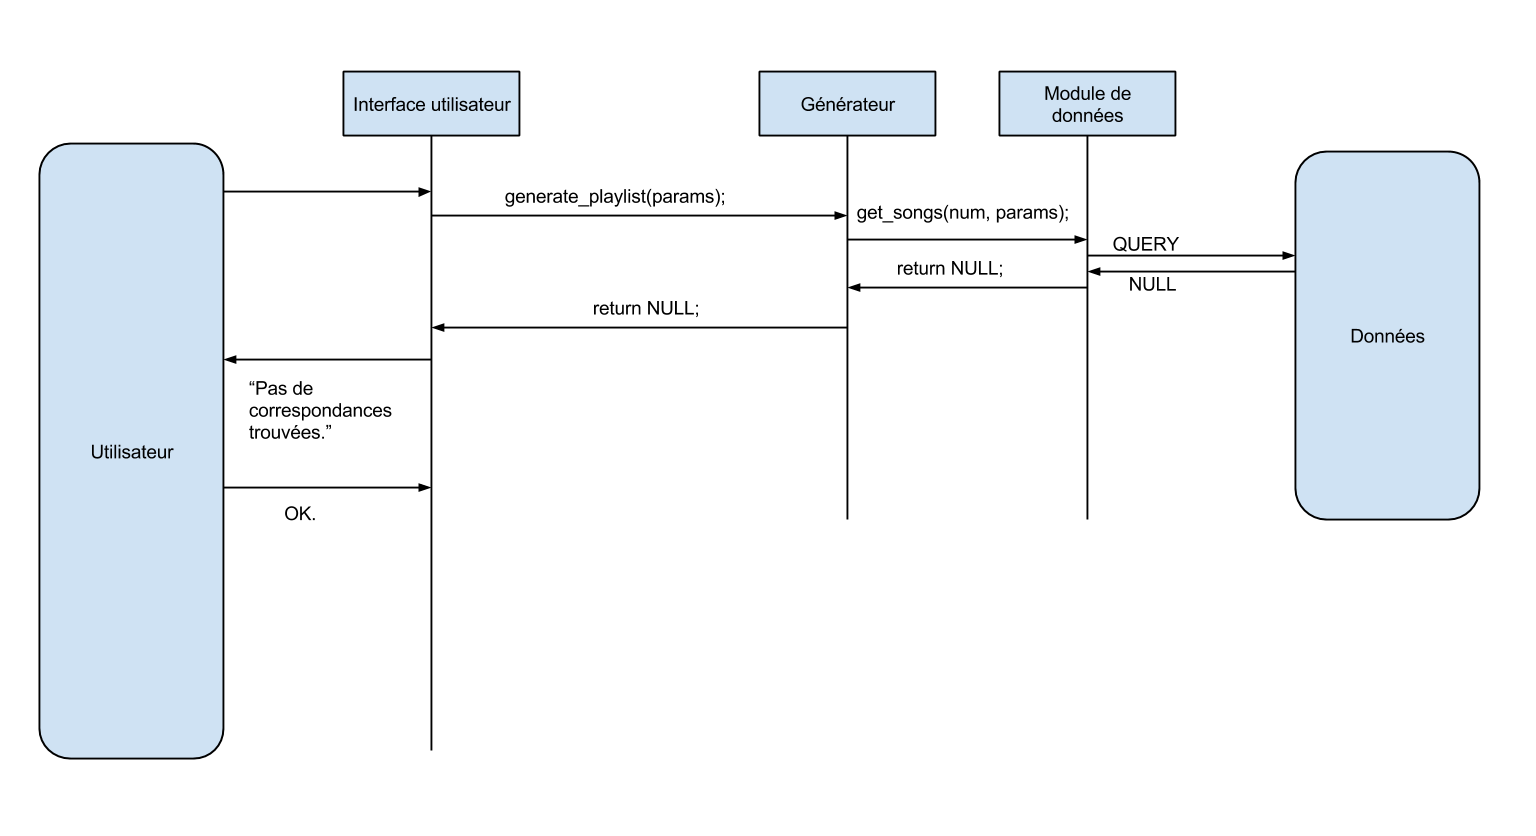
\includegraphics[width=\textwidth]{data/scenarii/generation_nulle.png}
\caption{Génération impossible, il n'y a pas de morceaux correspondants à la requête}
\end{figure}